% Created 2016-05-07 Sat 14:30
\documentclass[presentation,smaller]{beamer}
\usepackage[utf8]{inputenc}
\usepackage{fixltx2e}
\usepackage{graphicx}
\usepackage{grffile}
\usepackage{longtable}
\usepackage{wrapfig}
\usepackage{rotating}
\usepackage[normalem]{ulem}
\usepackage{amsmath}
\usepackage{textcomp}
\usepackage{amssymb}
\usepackage{capt-of}
\usepackage{hyperref}
\usepackage{color}
\usepackage{listings}
%
% Config
%

\usepackage{amsmath,amsfonts,amssymb,amsthm}
\usepackage{ifxetex,ifluatex}
\usepackage{fixltx2e} % provides \textsubscript
\usepackage{xspace}
\usepackage{graphicx}
\usepackage{comment}
\usepackage{url}
\usepackage{relsize}
\usepackage{booktabs}
\usepackage{tabularx}
\renewcommand*{\UrlFont}{\ttfamily\smaller\relax}
\usepackage{subfigure}
\usepackage[normalem]{ulem}
%
% Pseudocode
%

\usepackage[linesnumbered,ruled]{algorithm2e}

%
% Source Code Listings
%

\usepackage{listings}
\lstdefinelanguage{Sage}[]{Python}{morekeywords={True,False,sage,cdef,cpdef,ctypedef,self},sensitive=true}
\lstset{frame=none,
          showtabs=False,
          showspaces=False,
          showstringspaces=False,
          commentstyle={\color{gray}},
          keywordstyle={\color{mLightBrown}\textbf},
          stringstyle ={\color{mDarkBrown}},
          frame=single,
          basicstyle=\tt\scriptsize\relax,
          backgroundcolor=\color{gray!190!black},
          inputencoding=utf8,
          literate={…}{{\ldots}}1,
          belowskip=0.0em,
          }
\usepackage{lstlinebgrd}
%
% Tikz
%

% from pgfplotsthemetol.sty
\definecolor{DarkPurple}{HTML}{332288}
\definecolor{DarkBlue}{HTML}{6699CC}
\definecolor{LightBlue}{HTML}{88CCEE}
\definecolor{DarkGreen}{HTML}{117733}
\definecolor{DarkRed}{HTML}{661100}
\definecolor{LightRed}{HTML}{CC6677}
\definecolor{LightPink}{HTML}{AA4466}
\definecolor{DarkPink}{HTML}{882255}
\definecolor{LightPurple}{HTML}{AA4499}

\definecolor{DarkBrown}{HTML}{604c38}
\definecolor{DarkTeal}{HTML}{23373b}
\definecolor{LightBrown}{HTML}{EB811B}
\definecolor{LightGreen}{HTML}{14B03D}

\usepackage{tikz,pgfplots}
\usetikzlibrary{calc}
\usetikzlibrary{arrows,automata}
\usetikzlibrary{positioning}
\usetikzlibrary{decorations.pathmorphing}
\usetikzlibrary{decorations.pathreplacing}
\usetikzlibrary{backgrounds, fit, shapes.symbols, chains, shapes.geometric, shapes.arrows}
\usetikzlibrary{crypto.symbols}
\pgfplotsset{compat=1.12}
\usetikzlibrary{graphs}
\tikzset{shadows=no}

%% Cache TiKZ pictures

\ifdefined\tikzcaching
\usetikzlibrary{external}
\tikzexternalize[prefix=build/]
\tikzset{external/up to date check=diff} % MD5 fails from within emacs
\fi

%
% SVG

\ifxetex
\newcommand{\executeiffilenewer}[3]{%
 {\immediate\write18{#3}} % hack
}
\else
\newcommand{\executeiffilenewer}[3]{%
 \ifnum\pdfstrcmp{\pdffilemoddate{#1}}%
 {\pdffilemoddate{#2}}>0%
 {\immediate\write18{#3}}\fi%
}
\fi

\newcommand{\includesvg}[2][1.0\textwidth]{%
 \executeiffilenewer{#1.svg}{#1.pdf}%
 {inkscape -z -D --file=#2.svg --export-pdf=#2.pdf --export-latex --export-area-page}%
 \def\svgwidth{#1} 
 \input{#2.pdf_tex}%
} 

%
% Metropolis Theme
% https://github.com/matze/mtheme.git
%

\usetheme{metropolis}
\metroset{color/block=fill}
\metroset{numbering=none}
\metroset{outer/progressbar=foot}
\metroset{titleformat=smallcaps}


%
% UTF-8 all the things
% 
\usepackage{unicodesymbols} % put this after m which loads fontspec

%
% BibLaTeX
%

\usepackage[
    backend=bibtex,
    style=alphabetic,
    citestyle=alphabetic,
]{biblatex}

\bibliography{../local.bib, ../master_refs.bib, ../TLS.bib}

\DeclareFieldFormat{title}{\alert{#1}}
\DeclareFieldFormat[book]{title}{\alert{#1}}
\DeclareFieldFormat[inproceedings]{title}{\alert{#1}}
\DeclareFieldFormat[article]{title}{\alert{#1}}
\DeclareFieldFormat[misc]{title}{\alert{#1}}

%
% Microtype
%

\IfFileExists{upquote.sty}{\usepackage{upquote}}{}
\IfFileExists{microtype.sty}{\usepackage{microtype}}{}


\setlength{\parindent}{0pt}
\setlength{\parskip}{6pt plus 2pt minus 1pt}
\setlength{\emergencystretch}{3em}  % prevent overfull lines
\setcounter{secnumdepth}{0}


% \AtBeginSection[] 
% {
% \begin{frame}<beamer>
% \frametitle{Outline}
% \tableofcontents[currentsection]
% \end{frame}
% }

% \AtBeginSubsection[] 
% {
% \begin{frame}<beamer>
% \frametitle{Outline}
% \tableofcontents[currentsubsection]
% \end{frame}
% }

%%% Local Variables:
%%% mode: latex
%%% End:
\institute{Information Security Group, Royal Holloway, University of London}
\definecolor{ciphertext}{HTML}{F46D43}
\definecolor{sqn}{HTML}{CCCCCC}
\definecolor{diff}{HTML}{FEE08B}
\definecolor{plaintext}{HTML}{E6F598}
\definecolor{mac}{HTML}{FDAE61}
\definecolor{func}{HTML}{3288BD}
\usetheme{default}
\author{\alert{Martin R. Albrecht} and Kenny Paterson}
\date{Eurocrypt 2016}
\title{Lucky Microseconds}
\hypersetup{
 pdfauthor={\alert{Martin R. Albrecht} and Kenny Paterson},
 pdftitle={Lucky Microseconds},
 pdfkeywords={},
 pdfsubject={},
 pdfcreator={Emacs 24.5.1 (Org mode 8.3.4)}, 
 pdflang={English}}
\begin{document}

\maketitle

\begin{frame}[fragile,label={sec:orgheadline1}]{s2n}
 \begin{columns}
\begin{column}{0.6\columnwidth}
\begin{itemize}
\item \texttt{s2n} is a new implementation of TLS from Amazon Web Services (AWS).
\item Source code released on GitHub on 30 June 2015.
\item 6,000 lines of C instead of 70,000 lines in OpenSSL.
\item Three external security audits/code reviews were performed before release.
\end{itemize}
\end{column}

\begin{column}{0.4\columnwidth}

\includegraphics[width=.9\linewidth]{./s2n-eurocrypt-aws.png}


\includegraphics[width=.9\linewidth]{./s2n-eurocrypt-s2n.png}
\end{column}
\end{columns}
\end{frame}

\begin{frame}[label={sec:orgheadline2}]{s2n press at launch}
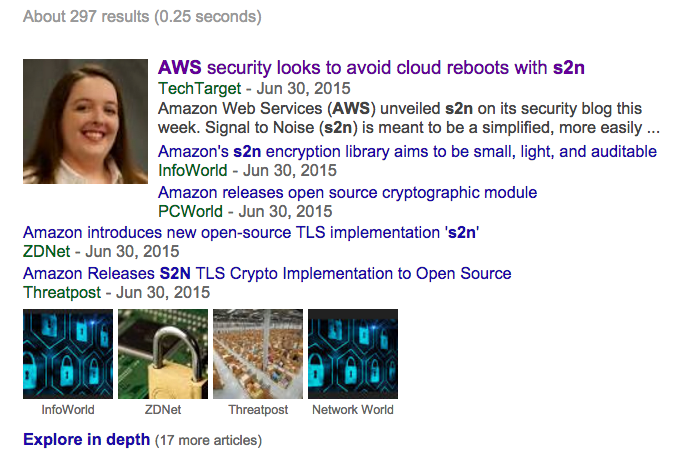
\includegraphics[width=.9\linewidth]{./s2n-eurocrypt-press.png}
\end{frame}

\begin{frame}[fragile,label={sec:orgheadline3}]{s2n and CBC-mode encryption}
 \begin{itemize}
\item \texttt{s2n} implements SSLv3 and TLS 1.0, 1.1 and 1.2.

\item So supports CBC-mode encryption.

\item Lucky 13:\footfullcite{AlFardan:2013a}

\begin{itemize}
\item Timing attack based on low-level internals of cryptographic processing for CBC-mode.
\end{itemize}

\item Countermeasures to Lucky 13 in OpenSSL needed 500 lines of code.

\item Can \texttt{s2n} be secure against Lucky 13 in just 6 kLoC?
\end{itemize}
\end{frame}

\begin{frame}[label={sec:orgheadline4}]{TLS Record Protocol: MAC-Encode-Encrypt (MEE)}
\begin{tikzpicture}[scale=0.66]
  \tikzstyle{sqn}=[fill=sqn]
  \tikzstyle{payload}=[fill=plaintext]
  \tikzstyle{func}=[fill=func]
  \tikzstyle{mac}=[fill=mac]
  \tikzstyle{padding}=[fill=diff]
  \tikzstyle{ciphertext}=[fill=ciphertext]
  \draw[sqn] (1,6) rectangle node{HDR} ++(2,1);
  \draw[ciphertext] (3,6) rectangle node[text=white]{Ciphertext} ++(13,1);

  \draw[thick,edge] (11,5) -- (12.5,5) -- (12.5,6);
  \draw[func] (8,4.5) rectangle node[text=white]{CBC} ++(3,1);
  \draw [decorate,decoration={brace,amplitude=6pt}]  (3,4) -- ++(13,0);

  \draw[payload] (3,3) rectangle node{Payload}++ (8,1);
  \draw[mac](11,3) rectangle node{MAC Tag} ++(3,1);
  \draw[padding](14,3) rectangle node{Padding} ++(2,1);

  \draw[thick,edge] (6.5,2) -- (12.5,2) -- (12.5,3);
  \draw[func] (3.5,1.5) rectangle node[text=white]{MAC} ++(3,1);
  \draw [decorate,decoration={brace,amplitude=6pt}]  (-1,1) -- ++(12,0) node [,midway,yshift=-0.8cm]  {};

  \draw[sqn] (-1,0) rectangle node{SQN$\Vert$HDR} ++(4,1);
  \draw[payload] (3,0) rectangle node{Payload}++ (8,1);
\end{tikzpicture}

\alert{Problem}: how to parse unauthenticated plaintext as payload, padding and MAC fields without leaking any information via error messages, timing or anything else?
\end{frame}


\begin{frame}[label={sec:orgheadline5}]{TLS Record Protocol: MAC-Encode-Encrypt (MEE)}
\begin{tikzpicture}[scale=0.66]
  \tikzstyle{sqn}=[fill=sqn]
  \tikzstyle{payload}=[fill=plaintext]
  \tikzstyle{func}=[fill=func]
  \tikzstyle{mac}=[fill=mac]
  \tikzstyle{padding}=[fill=diff]
  \tikzstyle{ciphertext}=[fill=ciphertext]
  \draw[sqn] (1,6) rectangle node{HDR} ++(2,1);
  \draw[ciphertext] (3,6) rectangle node[text=white]{Ciphertext} ++(13,1);

  \draw[thick,edge] (11,5) -- (12.5,5) -- (12.5,6);
  \draw[func] (8,4.5) rectangle node[text=white]{CBC} ++(3,1);
  \draw [decorate,decoration={brace,amplitude=6pt}]  (3,4) -- ++(13,0);

  \draw[payload] (3,3) rectangle node{Payload}++ (6,1);
  \draw[mac](9,3) rectangle node{MAC Tag} ++(3,1);
  \draw[padding](12,3) rectangle node{Padding} ++(4,1);

  \draw[thick,edge] (6.5,2) -- (10.5,2) -- (10.5,3);
  \draw[func] (3.5,1.5) rectangle node[text=white]{MAC} ++(3,1);
  \draw [decorate,decoration={brace,amplitude=6pt}]  (-1,1) -- ++(12,0) node [,midway,yshift=-0.8cm]  {};

  \draw[sqn] (-1,0) rectangle node{SQN$\Vert$HDR} ++(4,1);
  \draw[payload] (3,0) rectangle node{Payload}++ (8,1);
\end{tikzpicture}

\alert{Problem}: how to parse unauthenticated plaintext as payload, padding and MAC fields without leaking any information via error messages, timing or anything else?
\end{frame}

\begin{frame}[label={sec:orgheadline6}]{Constant Time Decryption for MEE}
\begin{itemize}
\item Lucky 13 exploits leakage from TLS's MEE decryption processing for CBC-mode.
\item Proper constant-time, constant-memory access implementation is needed to fully prevent it.
\item Hard when plaintext is a mix of unauthenticated padding, MAC and payload fragment.
\item See Adam Langley's blogpost\footnote{\url{https://www.imperialviolet.org/2013/02/04/luckythirteen.html}}
\end{itemize}

\begin{block}{TL;DR}
It’s hard to do it properly.
\end{block}
\end{frame}

\begin{frame}[fragile,label={sec:orgheadline7}]{It’s hard to do it properly, revisited (3/5/16)}
 \begin{tiny}

\begin{verbatim}
Padding oracle in AES-NI CBC MAC check (CVE-2016-2107)
======================================================

Severity: High

A MITM attacker can use a padding oracle attack to decrypt traffic
when the connection uses an AES CBC cipher and the server support
AES-NI.

This issue was introduced as part of the fix for Lucky 13 padding
attack (CVE-2013-0169). The padding check was rewritten to be in
constant time by making sure that always the same bytes are read and
compared against either the MAC or padding bytes. But it no longer
checked that there was enough data to have both the MAC and padding
bytes.

OpenSSL 1.0.2 users should upgrade to 1.0.2h
OpenSSL 1.0.1 users should upgrade to 1.0.1t

This issue was reported to OpenSSL on 13th of April 2016 by Juraj
Somorovsky using TLS-Attacker. The fix was developed by Kurt Roeckx
of the OpenSSL development team.
\end{verbatim}

\end{tiny}


\url{https://www.openssl.org/news/secadv/20160503.txt}
\url{https://github.com/RUB-NDS/TLS-Attacker}
\end{frame}

\begin{frame}[fragile,label={sec:orgheadline8}]{s2n and Lucky 13}
 The version of \texttt{s2n} we looked at protected against Lucky 13 using two countermeasures:

\begin{enumerate}
\item Dummy HMAC computations and padding checks to equalise running time.

\item Addition of random timing delays on decryption failure, to mask any residual timing differences.
\end{enumerate}
\end{frame}

\begin{frame}[fragile,label={sec:orgheadline9}]{\texttt{s2n\_verify\_cbc}}
 \lstset{language=C,label= ,caption= ,captionpos=b,numbers=none}
\begin{lstlisting}
int payload_and_padding_size = decrypted->size - mac_digest_size;

/* Determine what the padding length is */
uint8_t padding_length = decrypted->data[decrypted->size - 1];
\end{lstlisting}

\footnotesize Use the last byte of the last block to decide padding length.

\lstset{language=C,label= ,caption= ,captionpos=b,numbers=none}
\begin{lstlisting}
int payload_length = payload_and_padding_size - padding_length - 1;
\end{lstlisting}

Set \texttt{payload\_length} by subtracting this value from total size.

\lstset{language=C,label= ,caption= ,captionpos=b,numbers=none}
\begin{lstlisting}
/* Update the MAC */
GUARD(s2n_hmac_update(hmac, decrypted->data, payload_length));
\end{lstlisting}

Update MAC (but do not finalise), passing \texttt{payload\_length} bytes.
\end{frame}

\begin{frame}[fragile,label={sec:orgheadline10}]{\texttt{s2n\_verify\_cbc}}
 \lstset{language=C,label= ,caption= ,captionpos=b,numbers=none}
\begin{lstlisting}
GUARD(s2n_hmac_copy(&copy, hmac));
\end{lstlisting}

\footnotesize Make copy of HMAC data structure for later time equalisation.

\lstset{language=C,label= ,caption= ,captionpos=b,numbers=none}
\begin{lstlisting}
/* Check the MAC */
uint8_t check_digest[S2N_MAX_DIGEST_LEN];
lte_check(mac_digest_size, sizeof(check_digest));
GUARD(s2n_hmac_digest(hmac, check_digest, mac_digest_size));
\end{lstlisting}

Finalises MAC value.

Running time depends on value of \texttt{payload\_length}, which in turn depends on \texttt{padding\_length}, which \alert{might} leak plaintext information.
\end{frame}

\begin{frame}[fragile,label={sec:orgheadline11}]{\texttt{s2n\_verify\_cbc}}
 \lstset{language=C,label= ,caption= ,captionpos=b,numbers=none}
\begin{lstlisting}
int mismatches = s2n_constant_time_equals(decrypted->data
                                          + payload_length, check_digest,
                                          mac_digest_size) ^ 1;
\end{lstlisting}

\footnotesize Constant-time compare the computed HMAC value to the one extracted from \texttt{decrypted->data}.

\lstset{language=C,label= ,caption= ,captionpos=b,numbers=none}
\begin{lstlisting}
/* Compute a MAC on the rest of the data so that we perform
   the same number of hash operations */
GUARD(s2n_hmac_update(&copy,
                      decrypted->data + payload_length + mac_digest_size,
                      decrypted->size - payload_length - mac_digest_size
                         - 1));
\end{lstlisting}

Perform dummy \texttt{hmac\_update} operations to equalise running time of HMAC.
\end{frame}

\begin{frame}[label={sec:orgheadline12}]{Building Attack Ciphertext}
\begin{tikzpicture}[scale=0.64,every node/.style={scale=0.64}]
  \tikzstyle{ciphertext}=[draw,fill=ciphertext]
  \tikzstyle{plaintext}=[draw,fill=plaintext]

  \begin{scope}[xshift=-3cm]
    \draw[ciphertext](-2,-2)  rectangle node[text=white]{$IV$} ++(2,1);
    \draw[edge] (0,-1.5) -- (0.5, -1.5) -- (0.5,-4) -- (1.8,-4);
  \end{scope}

  \begin{scope}[xshift=0cm]
    \draw[ciphertext] (-2,-2)  rectangle node[text=white]{$R_1$} ++(2,1);
    \draw[thick] (-1,-2) -- (-1,-2.5);
    \draw (-1.5,-3.5) rectangle node{$D_{K}$} ++(1,1);
    \draw[thick] (-1,-3.5) -- (-1,-4.5);
    \node[XOR,thick] (x3) at (-1,-4) {};
    \draw[] (-2,-5.5)  rectangle node{} ++(2,1);
    \draw[edge] (0,-1.5) -- (0.5, -1.5) -- (0.5,-4) -- (1.8,-4);
  \end{scope}

  \begin{scope}[xshift=3cm]
    \draw[ciphertext] (-2,-2)  rectangle node[text=white]{$R_2$} ++(2,1);
    \draw[thick] (-1,-2) -- (-1,-2.5);
    \draw (-1.5,-3.5) rectangle node{$D_{K}$} ++(1,1);
    \draw[thick] (-1,-3.5) -- (-1,-4.5);
    \node[XOR,thick] (x3) at (-1,-4) {};
    \draw[] (-2,-5.5)  rectangle node{} ++(2,1);
    \draw[edge] (0,-1.5) -- (0.5, -1.5) -- (0.5,-4) -- (1.8,-4);
  \end{scope}

  \begin{scope}[xshift=6cm]
    \draw[ciphertext] (-2,-2)  rectangle node[text=white]{$R_3$} ++(2,1);
    \draw[thick] (-1,-2) -- (-1,-2.5);
    \draw (-1.5,-3.5) rectangle node{$D_{K}$} ++(1,1);
    \draw[thick] (-1,-3.5) -- (-1,-4.5);
    \node[XOR,thick] (x3) at (-1,-4) {};
    \draw[] (-2,-5.5)  rectangle node{} ++(2,1);
    \draw[edge] (0,-1.5) -- (0.5, -1.5) -- (0.5,-4) -- (1.8,-4);
  \end{scope}

  \begin{scope}[xshift=9cm]
    \draw[fill=diff,draw=none] (-3,-0.5)  rectangle node[]{XOR 1-byte $\Delta$ here} ++(4,1);
    \draw[ciphertext] (-2,-2)  rectangle node[text=white]{$C_{t-1}$} ++(2,1);
    \draw[fill=diff] (-0.25,-2) rectangle node {} ++(0.25,1);
    \draw[thick] (-1,-2) -- (-1,-2.5);
    \draw (-1.5,-3.5) rectangle node{$D_{K}$} ++(1,1);
    \draw[thick] (-1,-3.5) -- (-1,-4.5);
    \node[XOR,thick] (x3) at (-1,-4) {};
    \draw[] (-2,-5.5)  rectangle node{} ++(2,1);
    \draw[edge] (0,-1.5) -- (0.5, -1.5) -- (0.5,-4) -- (1.8,-4);
  \end{scope}

  \begin{scope}[xshift=12cm]
    \draw[ciphertext] (-2,-2)  rectangle node[text=white]{$C_{t}$} ++(2,1);
    \draw[thick] (-1,-2) -- (-1,-2.5);
    \draw (-1.5,-3.5) rectangle node{$D_{K}$} ++(1,1);
    \draw[thick] (-1,-3.5) -- (-1,-4.5);
    \node[XOR,thick] (x3) at (-1,-4) {};
    \draw[] (-2,-5.5)  rectangle node{} ++(2,1);
  \end{scope}

\end{tikzpicture}
\vspace{1cm}
\end{frame}

\begin{frame}[label={sec:orgheadline13}]{Case 1: last byte ≤ 4}
\begin{tikzpicture}[scale=0.64,every node/.style={scale=0.64}]
  \tikzstyle{ciphertext}=[draw,fill=ciphertext]
  \tikzstyle{plaintext}=[draw,fill=plaintext]

  \begin{scope}[xshift=-3cm]
    \draw[ciphertext](-2,-2)  rectangle node[text=white]{$IV$} ++(2,1);
    \draw[edge] (0,-1.5) -- (0.5, -1.5) -- (0.5,-4) -- (1.8,-4);
    \draw[fill=sqn] (-2,-5.5)  rectangle node{} ++(2,1);
  \end{scope}

  \begin{scope}[xshift=0cm]
    \draw[ciphertext] (-2,-2)  rectangle node[text=white]{$R_1$} ++(2,1);
    \draw[thick] (-1,-2) -- (-1,-2.5);
    \draw (-1.5,-3.5) rectangle node{$D_{K}$} ++(1,1);
    \draw[thick] (-1,-3.5) -- (-1,-4.5);
    \node[XOR,thick] (x3) at (-1,-4) {};
    \draw[plaintext] (-2,-5.5)  rectangle node{} ++(2,1);
    \draw[edge] (0,-1.5) -- (0.5, -1.5) -- (0.5,-4) -- (1.8,-4);
  \end{scope}

  \begin{scope}[xshift=3cm]
    \draw[ciphertext] (-2,-2)  rectangle node[text=white]{$R_2$} ++(2,1);
    \draw[thick] (-1,-2) -- (-1,-2.5);
    \draw (-1.5,-3.5) rectangle node{$D_{K}$} ++(1,1);
    \draw[thick] (-1,-3.5) -- (-1,-4.5);
    \node[XOR,thick] (x3) at (-1,-4) {};
    \draw[plaintext] (-2,-5.5)  rectangle node{} ++(2,1);
    \draw[edge] (0,-1.5) -- (0.5, -1.5) -- (0.5,-4) -- (1.8,-4);
  \end{scope}

  \begin{scope}[xshift=6cm]
    \draw[ciphertext] (-2,-2)  rectangle node[text=white]{$R_3$} ++(2,1);
    \draw[thick] (-1,-2) -- (-1,-2.5);
    \draw (-1.5,-3.5) rectangle node{$D_{K}$} ++(1,1);
    \draw[thick] (-1,-3.5) -- (-1,-4.5);
    \node[XOR,thick] (x3) at (-1,-4) {};
    \draw[plaintext] (-2,-5.5)  rectangle node{} ++(2,1);
    \draw[fill=mac] (-0.75,-5.5) rectangle node {} ++(0.75,1);
    \draw[edge] (0,-1.5) -- (0.5, -1.5) -- (0.5,-4) -- (1.8,-4);
  \end{scope}


  \begin{scope}[xshift=9cm]
    \draw[fill=diff,draw=none] (-3,-0.5)  rectangle node[]{XOR 1-byte $\Delta$ here} ++(4,1);
    \draw[ciphertext] (-2,-2)  rectangle node[text=white]{$C_{t-1}$} ++(2,1);
    \draw[fill=diff] (-0.25,-2) rectangle node {} ++(0.25,1);
    \draw[thick] (-1,-2) -- (-1,-2.5);
    \draw (-1.5,-3.5) rectangle node{$D_{K}$} ++(1,1);
    \draw[thick] (-1,-3.5) -- (-1,-4.5);
    \node[XOR,thick] (x3) at (-1,-4) {};
    \draw[fill=mac] (-2,-5.5)  rectangle node{} ++(2,1);
    \draw[edge] (0,-1.5) -- (0.5, -1.5) -- (0.5,-4) -- (1.8,-4);
  \end{scope}


  \begin{scope}[xshift=12cm]
    \draw[ciphertext] (-2,-2)  rectangle node[text=white]{$C_{t}$} ++(2,1);
    \draw[thick] (-1,-2) -- (-1,-2.5);
    \draw (-1.5,-3.5) rectangle node{$D_{K}$} ++(1,1);
    \draw[thick] (-1,-3.5) -- (-1,-4.5);
    \node[XOR,thick] (x3) at (-1,-4) {};
    \draw[fill=mac] (-2,-5.5)  rectangle node{} ++(2,1);
    \draw[fill=diff] (-0.75,-5.5) rectangle node {} ++(0.75,1);
  \end{scope}

  \draw [decorate,decoration={brace,amplitude=10pt,mirror}]
  (-5,-5.7) -- ++(10.2,0) node [black,midway,yshift=-0.8cm]
  {$\geq 13 + 16 + 16 + 11 = 56$  bytes};

  \draw [decorate,decoration={brace,amplitude=10pt,mirror}]
  (5.2,-5.7) -- ++(6.0,0) node [black,midway,yshift=-0.8cm]
  {$32$  bytes};

  \draw [decorate,decoration={brace,amplitude=3pt,mirror}]
  (11.2,-5.7) -- ++(0.80,0) node [black,midway,yshift=-0.8cm]
  {$\leq 5$  bytes};

  \draw[fill=diff,draw=none] (-3.3,-8.)  rectangle node[]{\textbf{5} SHA-256 compression function calls} ++(7.2,1);

  \draw[fill=diff,draw=none] (8,-8.0)  rectangle node[]{00, 01, 02, 03, 04} ++(3.5,1.0);
\end{tikzpicture}
\end{frame}

\begin{frame}[label={sec:orgheadline14}]{Case 2: last byte ≥ 5}
\begin{tikzpicture}[scale=0.64,every node/.style={scale=0.64}]
  \tikzstyle{ciphertext}=[draw,fill=ciphertext]
  \tikzstyle{plaintext}=[draw,fill=plaintext]

  \begin{scope}[xshift=-3cm]
    \draw[ciphertext](-2,-2)  rectangle node[text=white]{$IV$} ++(2,1);
    \draw[edge] (0,-1.5) -- (0.5, -1.5) -- (0.5,-4) -- (1.8,-4);
    \draw[fill=sqn] (-2,-5.5)  rectangle node{} ++(2,1);
  \end{scope}

  \begin{scope}[xshift=0cm]
    \draw[ciphertext] (-2,-2)  rectangle node[text=white]{$R_1$} ++(2,1);
    \draw[thick] (-1,-2) -- (-1,-2.5);
    \draw (-1.5,-3.5) rectangle node{$D_{K}$} ++(1,1);
    \draw[thick] (-1,-3.5) -- (-1,-4.5);
    \node[XOR,thick] (x3) at (-1,-4) {};
    \draw[plaintext] (-2,-5.5)  rectangle node{} ++(2,1);
    \draw[edge] (0,-1.5) -- (0.5, -1.5) -- (0.5,-4) -- (1.8,-4);
  \end{scope}

  \begin{scope}[xshift=3cm]
    \draw[ciphertext] (-2,-2)  rectangle node[text=white]{$R_2$} ++(2,1);
    \draw[thick] (-1,-2) -- (-1,-2.5);
    \draw (-1.5,-3.5) rectangle node{$D_{K}$} ++(1,1);
    \draw[thick] (-1,-3.5) -- (-1,-4.5);
    \node[XOR,thick] (x3) at (-1,-4) {};
    \draw[plaintext] (-2,-5.5)  rectangle node{} ++(2,1);
    \draw[edge] (0,-1.5) -- (0.5, -1.5) -- (0.5,-4) -- (1.8,-4);
  \end{scope}

  \begin{scope}[xshift=6cm]
    \draw[ciphertext] (-2,-2)  rectangle node[text=white]{$R_3$} ++(2,1);
    \draw[thick] (-1,-2) -- (-1,-2.5);
    \draw (-1.5,-3.5) rectangle node{$D_{K}$} ++(1,1);
    \draw[thick] (-1,-3.5) -- (-1,-4.5);
    \node[XOR,thick] (x3) at (-1,-4) {};
    \draw[plaintext] (-2,-5.5)  rectangle node{} ++(2,1);
    \draw[fill=mac] (-1.75,-5.5) rectangle node {} ++(1.75,1);
    \draw[edge] (0,-1.5) -- (0.5, -1.5) -- (0.5,-4) -- (1.8,-4);
  \end{scope}


  \begin{scope}[xshift=9cm]
    \draw[fill=diff,draw=none] (-3,-0.5)  rectangle node[]{XOR 1-byte $\Delta$ here} ++(4,1);
    \draw[ciphertext] (-2,-2)  rectangle node[text=white]{$C_{t-1}$} ++(2,1);
    \draw[fill=diff] (-0.25,-2) rectangle node {} ++(0.25,1);
    \draw[thick] (-1,-2) -- (-1,-2.5);
    \draw (-1.5,-3.5) rectangle node{$D_{K}$} ++(1,1);
    \draw[thick] (-1,-3.5) -- (-1,-4.5);
    \node[XOR,thick] (x3) at (-1,-4) {};
    \draw[fill=mac] (-2,-5.5)  rectangle node{} ++(2,1);
    \draw[edge] (0,-1.5) -- (0.5, -1.5) -- (0.5,-4) -- (1.8,-4);
  \end{scope}


  \begin{scope}[xshift=12cm]
    \draw[ciphertext] (-2,-2)  rectangle node[text=white]{$C_{t}$} ++(2,1);
    \draw[thick] (-1,-2) -- (-1,-2.5);
    \draw (-1.5,-3.5) rectangle node{$D_{K}$} ++(1,1);
    \draw[thick] (-1,-3.5) -- (-1,-4.5);
    \node[XOR,thick] (x3) at (-1,-4) {};
    \draw[fill=mac] (-2,-5.5)  rectangle node{} ++(2,1);
    \draw[fill=diff] (-1.75,-5.5) rectangle node {} ++(1.75,1);
  \end{scope}

  \draw [decorate,decoration={brace,amplitude=10pt,mirror}]
  (-5.0,-5.7) -- ++(9.2,0) node [black,midway,yshift=-0.8cm]
  {$\leq 13 + 16 + 16 + 10 = 55$  bytes};

  \draw [decorate,decoration={brace,amplitude=10pt,mirror}]
  (4.2,-5.7) -- ++(6.1,0) node [black,midway,yshift=-0.8cm]
  {$32$  bytes};

  \draw [decorate,decoration={brace,amplitude=8pt,mirror}]
  (10.3,-5.7) -- ++(1.70,0) node [black,midway,yshift=-0.8cm]
  {$\geq 6$  bytes};


  \draw[fill=diff,draw=none] (-3.3,-8.)  rectangle node[]{\textbf{4} SHA-256 compression function calls} ++(7.2,1);

  \draw[fill=diff,draw=none] (8,-8.0)  rectangle node[]{05, 06, 07, …, ff} ++(3.5,1.0);

\end{tikzpicture}
\end{frame}

\begin{frame}[fragile,label={sec:orgheadline15}]{Dummy HMAC computations in s2n}
 \begin{itemize}
\item There is a timing difference for the entire HMAC computation depending on whether the last byte is in \{\texttt{00}, \texttt{01}, \texttt{02}, \texttt{03}, \texttt{04}\} or in \{\texttt{05}, \texttt{06}, …, \texttt{ff}\}.
\item This last byte relates to the corresponding target plaintext byte in a controlled way.
\item The timing difference is of the same size as in the original Lucky 13 attack.
\end{itemize}

\alert{But what about that equalisation code, using dummy call to \texttt{hmac\_update}?}
\end{frame}

\begin{frame}[fragile,label={sec:orgheadline16}]{\texttt{s2n\_verify\_cbc}}
 \lstset{language=C,label= ,caption= ,captionpos=b,numbers=none}
\begin{lstlisting}
/* Compute a MAC on the rest of the data so that we perform
   the same number of hash operations */
GUARD(s2n_hmac_update(&copy,
                      decrypted->data + payload_length + mac_digest_size,
                      decrypted->size - payload_length - mac_digest_size
                         - 1));
\end{lstlisting}

\footnotesize For our ciphertexts, the input size is always 60 bytes. So \alert{zero} extra HMAC compression function computations are done, in either case.
\end{frame}

\begin{frame}[fragile,label={sec:orgheadline17}]{Experimental results: timing \texttt{s2n\_verify\_cbc}}
 \begin{center}
\begin{tabular}{rrrrrr}
Byte value & Cycles & Byte value & Cycles & Byte value & Cycles\\
\hline
\texttt{00} & 2251.96 & \texttt{05} & 1746.49 & … & …\\
\texttt{01} & 2354.57 & \texttt{06} & 1747.65 & \texttt{fc} & 1640.79\\
\texttt{02} & 2252.07 & \texttt{07} & 1705.62 & \texttt{fd} & 1634.61\\
\texttt{03} & 2135.11 & \texttt{08} & 1808.73 & \texttt{fe} & 1648.70\\
\texttt{04} & 2130.02 & \texttt{09} & 1806.50 & \texttt{ff} & 1634.64\\
\end{tabular}

\end{center}

Timing of function \texttt{s2n\_verify\_cbc} (in cycles) with \(H=\) \texttt{SHA-256} for different values of last byte in the \texttt{decrypted} buffer, each cycle count averaged over \(2^{8}\) trials.
\end{frame}

\begin{frame}[fragile,label={sec:orgheadline18}]{But wait… random timing delays in s2n!}
 \begin{itemize}
\item Addition of random timing delay in event of cryptographic processing error.
\item Intended to mask any residual timing differences from \texttt{s2n\_verify\_cbc}.
\item Time delay is a random value between 0 and 10 seconds.
\item Is that enough to mask a difference of \textasciitilde{}300 clock cycles?
\end{itemize}

\begin{block}{Textbook statistical analysis}
Trillions of samples would be needed to detect any timing differences if the delay was \alert{uniformly} random.
\end{block}
\end{frame}

\begin{frame}[fragile,label={sec:orgheadline19}]{Generating random timing delays in s2n}
 \lstset{language=C,label= ,caption= ,captionpos=b,numbers=none}
\begin{lstlisting}
if (s2n_record_parse(conn) < 0) {
    conn->closed = 1;
    GUARD(s2n_connection_wipe(conn));
\end{lstlisting}

\footnotesize Overwriting memory: varying time.

\lstset{language=C,label= ,caption= ,captionpos=b,numbers=none}
\begin{lstlisting}
    if (conn->blinding == S2N_BUILT_IN_BLINDING) {
        int delay;
        GUARD(delay = s2n_connection_get_delay(conn));
\end{lstlisting}

Generate random delay (uses calls to RNG + rejection sampling)

\lstset{language=C,label= ,caption= ,captionpos=b,numbers=none}
\begin{lstlisting}
        GUARD(sleep(delay / 1000000));
\end{lstlisting}

Sleep for at least number of seconds

\lstset{language=C,label= ,caption= ,captionpos=b,numbers=none}
\begin{lstlisting}
        GUARD(usleep(delay % 1000000));
    }
    return -1;
}
\end{lstlisting}

Sleep for at least number of microseconds
\end{frame}

\begin{frame}[fragile,label={sec:orgheadline20}]{Characterising the noise: \texttt{sleep()}}
 We can filter out any noise arising from \texttt{sleep(≥1)} calls by ignoring any delays larger than 1 second. Effect is to increase number of samples needed by factor of 10.

\begin{tikzpicture}
  \begin{axis}[width=0.9\textwidth,height=0.65\textheight,xlabel=clock cycles,xmin=0,xmax=500]
    \addplot[smooth,thick,mLightBrown,mark=] plot coordinates {
      (  0, 0.000) ( 10, 0.000) ( 20, 0.003) ( 30, 0.053) ( 40, 0.071)
      ( 50, 0.066) ( 60, 0.075) ( 70, 0.051) ( 80, 0.049) ( 90, 0.050)
      (100, 0.034) (110, 0.055) (120, 0.108) (130, 0.036) (140, 0.019)
      (150, 0.019) (160, 0.011) (170, 0.009) (180, 0.021) (190, 0.052)
      (200, 0.055) (210, 0.054) (220, 0.039) (230, 0.044) (240, 0.016)
      (250, 0.003) (260, 0.001) (270, 0.001) (280, 0.000) (290, 0.000)
      (300, 0.000) (310, 0.000) (320, 0.000) (330, 0.000) (340, 0.000)
      (350, 0.000) (360, 0.000) (370, 0.000) (380, 0.000) (390, 0.000)
      (400, 0.000) (410, 0.000) (420, 0.000) (430, 0.000) (440, 0.000)
      (450, 0.000) (460, 0.000) (470, 0.000) (480, 0.000) (490, 0.000)};
  \end{axis}
\end{tikzpicture}

\footnotesize Distribution of clock ticks for \texttt{sleep(0)} on Intel® Xeon® CPU E5-2667 v2 @ 3.30GHz.
\end{frame}

\begin{frame}[fragile,label={sec:orgheadline21}]{Characterising the noise: \texttt{usleep()}}
 \begin{quote}
The \texttt{usleep()} function suspends execution of the calling thread for (at least) usec microseconds. …
\end{quote}

The timing signal we are looking for is just a few hundred clock cycles. So take all timing measurements modulo 1 microsecond (3,300 clock cycles on test system).
\end{frame}

\begin{frame}[fragile,label={sec:orgheadline22}]{Characterising the noise: \texttt{usleep()}}
 \begin{quote}
The \texttt{usleep()} function suspends execution of the calling thread for (at least) usec microseconds. \alert{The sleep may be lengthened slightly by any system activity or by the time spent processing the call or by the granularity of system timers.}
\end{quote}

\texttt{usleep()} does not give a delay that is an exact number of microseconds, but has its own complex distribution.

\pause

However, despite this, \texttt{usleep()} does show exploitable non-uniform behaviour on the systems we tested.
\end{frame}

\begin{frame}[fragile,label={sec:orgheadline23}]{Characterising the noise: \texttt{usleep()}}
 \centering
\begin{tikzpicture}
  \begin{axis}[width=0.95\textwidth,
               height=0.65\textheight,
               xlabel=clock cycles,
               xmin=0, xmax=3300,
               ylabel=probability,
               legend entries={$d=10^3$, $d=10^4$, $d=10^5$,},
               legend pos= north east]
    \addplot[black,thick,mark=] plot coordinates {
      (   0, 0.01434) (  33, 0.01428) (  66, 0.01414) (  99, 0.01404) ( 132, 0.01393)
      ( 165, 0.01373) ( 198, 0.01353) ( 231, 0.01333) ( 264, 0.01315) ( 297, 0.01293)
      ( 330, 0.01269) ( 363, 0.01249) ( 396, 0.01230) ( 429, 0.01208) ( 462, 0.01188)
      ( 495, 0.01171) ( 528, 0.01150) ( 561, 0.01133) ( 594, 0.01113) ( 627, 0.01102)
      ( 660, 0.01088) ( 693, 0.01072) ( 726, 0.01063) ( 759, 0.01054) ( 792, 0.01043)
      ( 825, 0.01036) ( 858, 0.01031) ( 891, 0.01023) ( 924, 0.01019) ( 957, 0.01013)
      ( 990, 0.01004) (1023, 0.00997) (1056, 0.00989) (1089, 0.00978) (1122, 0.00968)
      (1155, 0.00959) (1188, 0.00950) (1221, 0.00937) (1254, 0.00923) (1287, 0.00909)
      (1320, 0.00901) (1353, 0.00888) (1386, 0.00878) (1419, 0.00869) (1452, 0.00858)
      (1485, 0.00848) (1518, 0.00840) (1551, 0.00829) (1584, 0.00817) (1617, 0.00803)
      (1650, 0.00792) (1683, 0.00778) (1716, 0.00767) (1749, 0.00753) (1782, 0.00743)
      (1815, 0.00731) (1848, 0.00720) (1881, 0.00710) (1914, 0.00701) (1947, 0.00692)
      (1980, 0.00682) (2013, 0.00675) (2046, 0.00671) (2079, 0.00667) (2112, 0.00668)
      (2145, 0.00666) (2178, 0.00672) (2211, 0.00678) (2244, 0.00690) (2277, 0.00704)
      (2310, 0.00719) (2343, 0.00741) (2376, 0.00765) (2409, 0.00789) (2442, 0.00814)
      (2475, 0.00838) (2508, 0.00862) (2541, 0.00883) (2574, 0.00904) (2607, 0.00920)
      (2640, 0.00938) (2673, 0.00947) (2706, 0.00960) (2739, 0.00975) (2772, 0.00991)
      (2805, 0.01009) (2838, 0.01033) (2871, 0.01063) (2904, 0.01095) (2937, 0.01132)
      (2970, 0.01174) (3003, 0.01215) (3036, 0.01259) (3069, 0.01296) (3102, 0.01337)
      (3135, 0.01368) (3168, 0.01394) (3201, 0.01413) (3234, 0.01427) (3267, 0.01437)};

    \addplot[mLightBrown,thick,mark=] plot coordinates {
      (   0, 0.00947) (  33, 0.00938) (  66, 0.00931) (  99, 0.00926) ( 132, 0.00919)
      ( 165, 0.00910) ( 198, 0.00903) ( 231, 0.00897) ( 264, 0.00890) ( 297, 0.00884)
      ( 330, 0.00880) ( 363, 0.00872) ( 396, 0.00869) ( 429, 0.00862) ( 462, 0.00860)
      ( 495, 0.00856) ( 528, 0.00851) ( 561, 0.00849) ( 594, 0.00847) ( 627, 0.00847)
      ( 660, 0.00847) ( 693, 0.00847) ( 726, 0.00851) ( 759, 0.00852) ( 792, 0.00859)
      ( 825, 0.00862) ( 858, 0.00869) ( 891, 0.00876) ( 924, 0.00881) ( 957, 0.00892)
      ( 990, 0.00896) (1023, 0.00903) (1056, 0.00913) (1089, 0.00917) (1122, 0.00926)
      (1155, 0.00937) (1188, 0.00944) (1221, 0.00952) (1254, 0.00962) (1287, 0.00972)
      (1320, 0.00986) (1353, 0.00997) (1386, 0.01007) (1419, 0.01021) (1452, 0.01034)
      (1485, 0.01046) (1518, 0.01054) (1551, 0.01065) (1584, 0.01076) (1617, 0.01082)
      (1650, 0.01087) (1683, 0.01094) (1716, 0.01101) (1749, 0.01106) (1782, 0.01113)
      (1815, 0.01117) (1848, 0.01125) (1881, 0.01130) (1914, 0.01139) (1947, 0.01146)
      (1980, 0.01149) (2013, 0.01157) (2046, 0.01162) (2079, 0.01163) (2112, 0.01168)
      (2145, 0.01163) (2178, 0.01158) (2211, 0.01153) (2244, 0.01152) (2277, 0.01142)
      (2310, 0.01135) (2343, 0.01132) (2376, 0.01123) (2409, 0.01119) (2442, 0.01115)
      (2475, 0.01110) (2508, 0.01107) (2541, 0.01103) (2574, 0.01099) (2607, 0.01095)
      (2640, 0.01088) (2673, 0.01079) (2706, 0.01069) (2739, 0.01058) (2772, 0.01048)
      (2805, 0.01035) (2838, 0.01023) (2871, 0.01013) (2904, 0.01003) (2937, 0.00991)
      (2970, 0.00983) (3003, 0.00981) (3036, 0.00972) (3069, 0.00968) (3102, 0.00966)
      (3135, 0.00965) (3168, 0.00963) (3201, 0.00960) (3234, 0.00956) (3267, 0.00951)
    };

    \addplot[very thick,lightgray,mark=] plot coordinates {
      (   0, 0.01057) (  33, 0.01049) (  66, 0.01043) (  99, 0.01038) ( 132, 0.01033)
      ( 165, 0.01022) ( 198, 0.01014) ( 231, 0.01007) ( 264, 0.01000) ( 297, 0.00993)
      ( 330, 0.00985) ( 363, 0.00975) ( 396, 0.00967) ( 429, 0.00961) ( 462, 0.00956)
      ( 495, 0.00948) ( 528, 0.00942) ( 561, 0.00935) ( 594, 0.00927) ( 627, 0.00922)
      ( 660, 0.00915) ( 693, 0.00909) ( 726, 0.00905) ( 759, 0.00897) ( 792, 0.00894)
      ( 825, 0.00888) ( 858, 0.00883) ( 891, 0.00879) ( 924, 0.00876) ( 957, 0.00871)
      ( 990, 0.00870) (1023, 0.00867) (1056, 0.00865) (1089, 0.00862) (1122, 0.00861)
      (1155, 0.00860) (1188, 0.00861) (1221, 0.00859) (1254, 0.00860) (1287, 0.00860)
      (1320, 0.00864) (1353, 0.00865) (1386, 0.00866) (1419, 0.00870) (1452, 0.00874)
      (1485, 0.00880) (1518, 0.00883) (1551, 0.00890) (1584, 0.00895) (1617, 0.00902)
      (1650, 0.00912) (1683, 0.00920) (1716, 0.00927) (1749, 0.00935) (1782, 0.00944)
      (1815, 0.00956) (1848, 0.00967) (1881, 0.00974) (1914, 0.00986) (1947, 0.00996)
      (1980, 0.01008) (2013, 0.01022) (2046, 0.01035) (2079, 0.01046) (2112, 0.01061)
      (2145, 0.01071) (2178, 0.01085) (2211, 0.01095) (2244, 0.01108) (2277, 0.01118)
      (2310, 0.01127) (2343, 0.01133) (2376, 0.01141) (2409, 0.01144) (2442, 0.01150)
      (2475, 0.01152) (2508, 0.01155) (2541, 0.01155) (2574, 0.01156) (2607, 0.01153)
      (2640, 0.01156) (2673, 0.01151) (2706, 0.01150) (2739, 0.01146) (2772, 0.01143)
      (2805, 0.01141) (2838, 0.01138) (2871, 0.01127) (2904, 0.01122) (2937, 0.01118)
      (2970, 0.01113) (3003, 0.01107) (3036, 0.01103) (3069, 0.01095) (3102, 0.01091)
      (3135, 0.01085) (3168, 0.01080) (3201, 0.01072) (3234, 0.01066) (3267, 0.01061)
    };
  \end{axis}
  \end{tikzpicture}

\footnotesize Distribution of clock ticks modulo 3,300 for \texttt{usleep(delay)} with \texttt{delay} uniformly random in \(\left[0,d\right)\).
\end{frame}

\begin{frame}[label={sec:orgheadline24}]{Characterising the noise: wiping \& random sampling}
\begin{tikzpicture}
  \begin{axis}[width=0.95\textwidth,
              height=0.7\textheight,
              xlabel=clock cycles,
              ylabel=probability,
              xmin=0,xmax=3300,
              legend entries={\lstinline{s2n_stuffer_wipe}, \lstinline{s2n_public_random}},
              legend pos= north east]
    \addplot[smooth,thick,mLightBrown,mark=] plot coordinates {
      (  0, 0.000) ( 10, 0.000) ( 20, 0.000) ( 30, 0.000) ( 40, 0.000)
      ( 50, 0.000) ( 60, 0.000) ( 70, 0.000) ( 80, 0.000) ( 90, 0.000)
      (100, 0.000) (110, 0.000) (120, 0.000) (130, 0.001) (140, 0.005)
      (150, 0.031) (160, 0.045) (170, 0.026) (180, 0.034) (190, 0.034)
      (200, 0.027) (210, 0.033) (220, 0.028) (230, 0.027) (240, 0.028)
      (250, 0.019) (260, 0.019) (270, 0.018) (280, 0.012) (290, 0.011)
      (300, 0.011) (310, 0.008) (320, 0.008) (330, 0.014) (340, 0.011)
      (350, 0.012) (360, 0.022) (370, 0.016) (380, 0.016) (390, 0.024)
      (400, 0.016) (410, 0.015) (420, 0.020) (430, 0.013) (440, 0.020)
      (450, 0.037) (460, 0.018) (470, 0.014) (480, 0.014) (490, 0.007)
      (500, 0.005) (510, 0.006) (520, 0.004) (530, 0.003) (540, 0.004)
      (550, 0.007) (560, 0.014) (570, 0.047) (580, 0.050) (590, 0.058)
      (600, 0.051) (610, 0.019) (620, 0.007) (630, 0.004) (640, 0.001)
      (650, 0.001) (660, 0.001) (670, 0.000) (680, 0.000) (690, 0.000)
      (700, 0.000) (710, 0.000) (720, 0.000) (730, 0.000) (740, 0.000)
      (750, 0.000) (760, 0.000) (770, 0.000) (780, 0.000) (790, 0.000)
      (3267, 0.000)};

    \addplot[thick, smooth,black,mark=] plot coordinates {
      (   0, 0.008) (  33, 0.008) (  66, 0.008) (  99, 0.008) ( 132, 0.008)
      ( 165, 0.008) ( 198, 0.008) ( 231, 0.008) ( 264, 0.008) ( 297, 0.007)
      ( 330, 0.007) ( 363, 0.007) ( 396, 0.007) ( 429, 0.007) ( 462, 0.007)
      ( 495, 0.007) ( 528, 0.008) ( 561, 0.008) ( 594, 0.009) ( 627, 0.011)
      ( 660, 0.011) ( 693, 0.011) ( 726, 0.011) ( 759, 0.010) ( 792, 0.009)
      ( 825, 0.008) ( 858, 0.007) ( 891, 0.006) ( 924, 0.005) ( 957, 0.004)
      ( 990, 0.003) (1023, 0.003) (1056, 0.002) (1089, 0.002) (1122, 0.002)
      (1155, 0.001) (1188, 0.001) (1221, 0.001) (1254, 0.001) (1287, 0.001)
      (1320, 0.001) (1353, 0.001) (1386, 0.001) (1419, 0.001) (1452, 0.001)
      (1485, 0.002) (1518, 0.002) (1551, 0.003) (1584, 0.004) (1617, 0.006)
      (1650, 0.008) (1683, 0.010) (1716, 0.013) (1749, 0.016) (1782, 0.021)
      (1815, 0.026) (1848, 0.031) (1881, 0.035) (1914, 0.037) (1947, 0.037)
      (1980, 0.035) (2013, 0.030) (2046, 0.026) (2079, 0.022) (2112, 0.019)
      (2145, 0.015) (2178, 0.013) (2211, 0.012) (2244, 0.012) (2277, 0.012)
      (2310, 0.013) (2343, 0.014) (2376, 0.014) (2409, 0.013) (2442, 0.013)
      (2475, 0.012) (2508, 0.012) (2541, 0.011) (2574, 0.010) (2607, 0.010)
      (2640, 0.009) (2673, 0.009) (2706, 0.008) (2739, 0.009) (2772, 0.009)
      (2805, 0.009) (2838, 0.009) (2871, 0.009) (2904, 0.009) (2937, 0.008)
      (2970, 0.008) (3003, 0.009) (3036, 0.009) (3069, 0.009) (3102, 0.008)
      (3135, 0.008) (3168, 0.008) (3201, 0.008) (3234, 0.007) (3267, 0.007)
    };
  \end{axis}
\end{tikzpicture}

\footnotesize Distribution of clock ticks modulo 3,300.
\end{frame}
\begin{frame}[label={sec:orgheadline25}]{Random timing delays in s2n}
\begin{tikzpicture}
  \begin{axis}[width=0.95\textwidth,height=0.7\textheight,xlabel=clock cycles,ylabel=probability,xmin=0,xmax=3300, legend entries={{\tt 00}, {\tt 05}}, legend pos=north west]
    \addplot[thick,smooth,black,mark=] plot coordinates {
      (   0, 0.01002) (  33, 0.00997) (  66, 0.00996) (  99, 0.00994) ( 132, 0.00989)
      ( 165, 0.00987) ( 198, 0.00982) ( 231, 0.00980) ( 264, 0.00980) ( 297, 0.00975)
      ( 330, 0.00971) ( 363, 0.00966) ( 396, 0.00967) ( 429, 0.00962) ( 462, 0.00960)
      ( 495, 0.00956) ( 528, 0.00956) ( 561, 0.00953) ( 594, 0.00949) ( 627, 0.00948)
      ( 660, 0.00947) ( 693, 0.00944) ( 726, 0.00945) ( 759, 0.00943) ( 792, 0.00942)
      ( 825, 0.00942) ( 858, 0.00944) ( 891, 0.00943) ( 924, 0.00944) ( 957, 0.00943)
      ( 990, 0.00945) (1023, 0.00947) (1056, 0.00949) (1089, 0.00950) (1122, 0.00952)
      (1155, 0.00954) (1188, 0.00957) (1221, 0.00959) (1254, 0.00962) (1287, 0.00968)
      (1320, 0.00973) (1353, 0.00975) (1386, 0.00980) (1419, 0.00983) (1452, 0.00987)
      (1485, 0.00992) (1518, 0.00996) (1551, 0.00999) (1584, 0.01002) (1617, 0.01008)
      (1650, 0.01012) (1683, 0.01015) (1716, 0.01019) (1749, 0.01021) (1782, 0.01025)
      (1815, 0.01026) (1848, 0.01030) (1881, 0.01032) (1914, 0.01035) (1947, 0.01035)
      (1980, 0.01038) (2013, 0.01040) (2046, 0.01041) (2079, 0.01039) (2112, 0.01042)
      (2145, 0.01043) (2178, 0.01044) (2211, 0.01044) (2244, 0.01044) (2277, 0.01045)
      (2310, 0.01044) (2343, 0.01045) (2376, 0.01045) (2409, 0.01046) (2442, 0.01047)
      (2475, 0.01046) (2508, 0.01043) (2541, 0.01047) (2574, 0.01045) (2607, 0.01044)
      (2640, 0.01042) (2673, 0.01041) (2706, 0.01043) (2739, 0.01040) (2772, 0.01037)
      (2805, 0.01036) (2838, 0.01034) (2871, 0.01030) (2904, 0.01034) (2937, 0.01030)
      (2970, 0.01028) (3003, 0.01025) (3036, 0.01024) (3069, 0.01021) (3102, 0.01020)
      (3135, 0.01014) (3168, 0.01013) (3201, 0.01010) (3234, 0.01008) (3267, 0.01006)
    };
    \addplot[smooth,mLightBrown,thick,mark=] plot coordinates {
      (   0, 0.00923) (  33, 0.00925) (  66, 0.00927) (  99, 0.00927) ( 132, 0.00930)
      ( 165, 0.00930) ( 198, 0.00932) ( 231, 0.00936) ( 264, 0.00941) ( 297, 0.00943)
      ( 330, 0.00947) ( 363, 0.00952) ( 396, 0.00956) ( 429, 0.00961) ( 462, 0.00966)
      ( 495, 0.00972) ( 528, 0.00979) ( 561, 0.00983) ( 594, 0.00990) ( 627, 0.00994)
      ( 660, 0.01002) ( 693, 0.01008) ( 726, 0.01013) ( 759, 0.01016) ( 792, 0.01023)
      ( 825, 0.01026) ( 858, 0.01031) ( 891, 0.01036) ( 924, 0.01040) ( 957, 0.01044)
      ( 990, 0.01047) (1023, 0.01053) (1056, 0.01053) (1089, 0.01058) (1122, 0.01060)
      (1155, 0.01063) (1188, 0.01065) (1221, 0.01066) (1254, 0.01066) (1287, 0.01066)
      (1320, 0.01069) (1353, 0.01069) (1386, 0.01067) (1419, 0.01069) (1452, 0.01069)
      (1485, 0.01068) (1518, 0.01068) (1551, 0.01067) (1584, 0.01066) (1617, 0.01066)
      (1650, 0.01062) (1683, 0.01064) (1716, 0.01060) (1749, 0.01060) (1782, 0.01056)
      (1815, 0.01054) (1848, 0.01051) (1881, 0.01048) (1914, 0.01046) (1947, 0.01042)
      (1980, 0.01038) (2013, 0.01038) (2046, 0.01037) (2079, 0.01031) (2112, 0.01027)
      (2145, 0.01023) (2178, 0.01023) (2211, 0.01017) (2244, 0.01015) (2277, 0.01011)
      (2310, 0.01010) (2343, 0.01001) (2376, 0.01000) (2409, 0.00994) (2442, 0.00991)
      (2475, 0.00986) (2508, 0.00984) (2541, 0.00980) (2574, 0.00974) (2607, 0.00970)
      (2640, 0.00964) (2673, 0.00965) (2706, 0.00959) (2739, 0.00958) (2772, 0.00953)
      (2805, 0.00950) (2838, 0.00944) (2871, 0.00943) (2904, 0.00939) (2937, 0.00937)
      (2970, 0.00934) (3003, 0.00933) (3036, 0.00930) (3069, 0.00929) (3102, 0.00927)
      (3135, 0.00924) (3168, 0.00924) (3201, 0.00921) (3234, 0.00923) (3267, 0.00922)
    };
  \end{axis}
\end{tikzpicture}

\footnotesize Distribution of clock ticks modulo 3,300 for timing signals with the maximum delay restricted to \(d=100,000\).
\end{frame}

\begin{frame}[fragile,label={sec:orgheadline26}]{Putting it all together}
 \begin{itemize}
\item Kullback–Leibler divergence: \(3.6 × 10^{-3}\).

\item Hence about 280 ciphertexts are needed to distinguish \texttt{00} from \texttt{05}, for max delay \(100,000 μs\).

\item 28k ciphertexts for real delay of \(10s\).

\item Extends to plaintext recovery attack using a standard maximum likelihood based approach.

\item More samples are needed because now we are trying to identify one correct value amongst 255 wrong values.
\end{itemize}
\end{frame}

\begin{frame}[fragile,label={sec:orgheadline27}]{Disclosure and interaction with AWS}
 \begin{itemize}
\item \texttt{s2n} was released on June 30th 2015.
\item We informed the AWS team about the HMAC processing error in \texttt{s2n\_verify\_cbc} on July 5th 2015.
\item AWS patched the \texttt{s2n} code almost immediately.
\item They also informed us about their random timing delay countermeasure, which prompted our study of this countermeasure.
\item Meanwhile, \texttt{s2n} switched to using \texttt{nanosleep()}.
\item Disclosure process was very smooth.
\end{itemize}
\end{frame}

\begin{frame}[fragile,label={sec:orgheadline28}]{\texttt{nanonsleep()}}
 \begin{itemize}
\item Our experiments indicate that the distribution of \texttt{nanonsleep()} as implemented on Linux is sufficiently close to uniform to thwart the attack.
\item However, relying on it puts a high security burden on this function which is not designed for this purpose.
\end{itemize}

\begin{quote}
\texttt{nanosleep()} suspends the execution of the calling thread until either \alert{at least} the time specified in \texttt{*req} has elapsed, or the delivery of a signal that triggers the invocation of a handler in the calling thread or that terminates the process.
\end{quote}
\end{frame}

\begin{frame}[label={sec:orgheadline29}]{Takeaways}
\begin{itemize}
\item Lucky 13 is hard to fully protect against.
\item OpenSSL does it, but the code is not transparent → CVE-2016-2107
\item MEE makes it hard to produce secure implementations, it should be phased out as soon as possible.
\item Pre-release code audits will not catch all subtle crypto flaws.
\item AWS invited public analysis of their code and reacted well to our work.
\end{itemize}
\end{frame}

\begin{frame}[label={sec:orgheadline30}]{Fin}
\begin{center}
\begin{Huge}
\alert{Thank You}
\end{Huge}
\end{center}

\alert{s2n} \url{https://github.com/awslabs/s2n}

\alert{Paper} \url{http://ia.cr/2015/1129}

\alert{Press} \url{http://arstechnica.com/science/2015/11/researchers-poke}

\alert{AWS Blog} \url{https://blogs.aws.amazon.com/security/blog/tag/s2n}
\end{frame}
\end{document}